\documentclass[journal,12pt,twocolumn]{IEEEtran}

\usepackage{setspace}
\usepackage{gensymb}
\singlespacing
\usepackage[cmex10]{amsmath}

\usepackage{amsthm}

\usepackage{mathrsfs}
\usepackage{txfonts}
\usepackage{stfloats}
\usepackage{bm}
\usepackage{cite}
\usepackage{cases}
\usepackage{subfig}

\usepackage{longtable}
\usepackage{multirow}

\usepackage{enumitem}
\usepackage{mathtools}
\usepackage{steinmetz}
\usepackage{tikz}
\usepackage{circuitikz}
\usepackage{verbatim}
\usepackage{tfrupee}
\usepackage[breaklinks=true]{hyperref}
\usepackage{graphicx}
\usepackage{tkz-euclide}

\usetikzlibrary{calc,math}
\usepackage{listings}
    \usepackage{color}                                            %%
    \usepackage{array}                                            %%
    \usepackage{longtable}                                        %%
    \usepackage{calc}                                             %%
    \usepackage{multirow}                                         %%
    \usepackage{hhline}                                           %%
    \usepackage{ifthen}                                           %%
    \usepackage{lscape}     
\usepackage{multicol}
\usepackage{chngcntr}

\DeclareMathOperator*{\Res}{Res}

\renewcommand\thesection{\arabic{section}}
\renewcommand\thesubsection{\thesection.\arabic{subsection}}
\renewcommand\thesubsubsection{\thesubsection.\arabic{subsubsection}}

\renewcommand\thesectiondis{\arabic{section}}
\renewcommand\thesubsectiondis{\thesectiondis.\arabic{subsection}}
\renewcommand\thesubsubsectiondis{\thesubsectiondis.\arabic{subsubsection}}


\hyphenation{op-tical net-works semi-conduc-tor}
\def\inputGnumericTable{}                                 %%

\lstset{
%language=C,
frame=single, 
breaklines=true,
columns=fullflexible
}
\begin{document}

\newcommand{\BEQA}{\begin{eqnarray}}
\newcommand{\EEQA}{\end{eqnarray}}
\newcommand{\define}{\stackrel{\triangle}{=}}
\bibliographystyle{IEEEtran}
\raggedbottom
\setlength{\parindent}{0pt}
\providecommand{\mbf}{\mathbf}
\providecommand{\pr}[1]{\ensuremath{\Pr\left(#1\right)}}
\providecommand{\qfunc}[1]{\ensuremath{Q\left(#1\right)}}
\providecommand{\sbrak}[1]{\ensuremath{{}\left[#1\right]}}
\providecommand{\lsbrak}[1]{\ensuremath{{}\left[#1\right.}}
\providecommand{\rsbrak}[1]{\ensuremath{{}\left.#1\right]}}
\providecommand{\brak}[1]{\ensuremath{\left(#1\right)}}
\providecommand{\lbrak}[1]{\ensuremath{\left(#1\right.}}
\providecommand{\rbrak}[1]{\ensuremath{\left.#1\right)}}
\providecommand{\cbrak}[1]{\ensuremath{\left\{#1\right\}}}
\providecommand{\lcbrak}[1]{\ensuremath{\left\{#1\right.}}
\providecommand{\rcbrak}[1]{\ensuremath{\left.#1\right\}}}
\theoremstyle{remark}
\newtheorem{rem}{Remark}
\newcommand{\sgn}{\mathop{\mathrm{sgn}}}
\providecommand{\abs}[1]{\vert#1\vert}
\providecommand{\res}[1]{\Res\displaylimits_{#1}} 
\providecommand{\norm}[1]{\lVert#1\rVert}
%\providecommand{\norm}[1]{\lVert#1\rVert}
\providecommand{\mtx}[1]{\mathbf{#1}}
\providecommand{\mean}[1]{E[ #1 ]}
\providecommand{\fourier}{\overset{\mathcal{F}}{ \rightleftharpoons}}
%\providecommand{\hilbert}{\overset{\mathcal{H}}{ \rightleftharpoons}}
\providecommand{\system}{\overset{\mathcal{H}}{ \longleftrightarrow}}
	%\newcommand{\solution}[2]{\textbf{Solution:}{#1}}
\newcommand{\solution}{\noindent \textbf{Solution: }}
\newcommand{\cosec}{\,\text{cosec}\,}
\providecommand{\dec}[2]{\ensuremath{\overset{#1}{\underset{#2}{\gtrless}}}}
\newcommand{\myvec}[1]{\ensuremath{\begin{pmatrix}#1\end{pmatrix}}}
\newcommand{\mydet}[1]{\ensuremath{\begin{vmatrix}#1\end{vmatrix}}}
\numberwithin{equation}{subsection}
\makeatletter
\@addtoreset{figure}{problem}
\makeatother
\let\StandardTheFigure\thefigure
\let\vec\mathbf
\renewcommand{\thefigure}{\theproblem}
\def\putbox#1#2#3{\makebox[0in][l]{\makebox[#1][l]{}\raisebox{\baselineskip}[0in][0in]{\raisebox{#2}[0in][0in]{#3}}}}
     \def\rightbox#1{\makebox[0in][r]{#1}}
     \def\centbox#1{\makebox[0in]{#1}}
     \def\topbox#1{\raisebox{-\baselineskip}[0in][0in]{#1}}
     \def\midbox#1{\raisebox{-0.5\baselineskip}[0in][0in]{#1}}
\vspace{3cm}
\title{Assignment 2}
\author{Chirag Mehta - AI20BTECH11006}
\maketitle
\newpage
\bigskip
\renewcommand{\thefigure}{\theenumi}
\renewcommand{\thetable}{\theenumi}
Download all python codes from 
\begin{lstlisting}
https://github.com/cmapsi/AI1103-Probability-and-random-variables/tree/main/Assignment-2/codes
\end{lstlisting}
and latex-tikz codes from 
\begin{lstlisting}
https://github.com/cmapsi/AI1103-Probability-and-random-variables/blob/main/Assignment-2/main.tex
\end{lstlisting}
\section{Problem}
Two dice, one blue and one grey, are thrown at the same time. Write down all the possible outcomes.What is the probability that the sum of the two numbers appearing on the top of the dice is\\
(i) 8?\\
(ii) 13?\\
(iii) less than or equal to 12?
\section{solution}

Let $X_i \in \{1,2,3,4,5,6\},\ i=1,2$ be the random variables representing the outcomes of each die.
The probability mass function is given below.
\begin{align}
\label{eq:outcomes}
p_{X_i}(n) = \pr{X_i = n} = 
\begin{cases}
\frac{1}{6} & 1 \le n \le 6
\\
0 & otherwise
\end{cases}
\end{align}
Desired outcomes
\begin{align}
X=X_1+X_2=n
\end{align}
\begin{align}
	p_X(n)=\Pr{(X_1+X_2=n)}=\Pr{(X_1=n-X_2)}\\
	=\displaystyle \sum_k \Pr{(X_1=n-k|X_2=k)}p_{X_2}(k) \label{eq:sum}
\end{align}
Since $X_1$ and $X_2$ are independents events, we can deduce
\begin{align}
\Pr{(X_1=n-k|X_2=k)}=\Pr{(X_1=n-k)}=p_{X_1}(n-k)
\label{eq:independent}
\end{align}

From \eqref{eq:sum} and \eqref{eq:independent}
\begin{align}
	p_X(n)=\displaystyle \sum_k p_{X_1}(n-k)p_{X_2}
	=p_{X_1}(n)*p_{X_2}(n)
\label{eq:convo}
\end{align}
From \eqref{eq:outcomes} and \eqref{eq:convo}
\begin{align}
	p_X(n)=\dfrac{1}{6}\displaystyle \sum_{k=1}^6 {p_{X_1}(n-k)}	
\end{align}
\begin{align}
	p_{X_1}(k)=0\text{, if } k\notin{\{1,2,3,4,5,6\}}
\end{align}
\begin{align}
p_X(n) &= 
\begin{cases}
0 & n < 1\\
\frac{1}{6}\sum_{k=1}^{n-1}p_{X_1}(k) &  1 \le n-1 \le  6\\
\frac{1}{6}\sum_{k=n-6}^{6}p_{X_1}(k) & 1 < n-6 \le 6\\
0 & n > 12
\end{cases}
\end{align}
Since,
\begin{align}
	p_{X_1}(k)=0\text{, if } k\notin{\{1,2,3,4,5,6\}}
\end{align}
We can reduce it to
\begin{align}
	p_X(n) &=
\begin{cases}
0 & n < 1\\
\frac{n-1}{36} &  2 \le n \le  7 \\
\frac{13-n}{36} & 7 < n \le 12 \\
0 & n > 12
\end{cases}
\label{eq:final_result}
\end{align}

Using \eqref{eq:final_result} we get the following answers

\begin{center}
  
  \begin{tabular}{|c|c|c|c|}
    \hline
    case &  sum=8 & sum=13 & $sum\leq 12$\\
    \hline
    \pr{n} & 0.138889 & 0& 1\\
    \hline
    
\end{tabular}
\end{center}
\newpage
The graph in given below\\
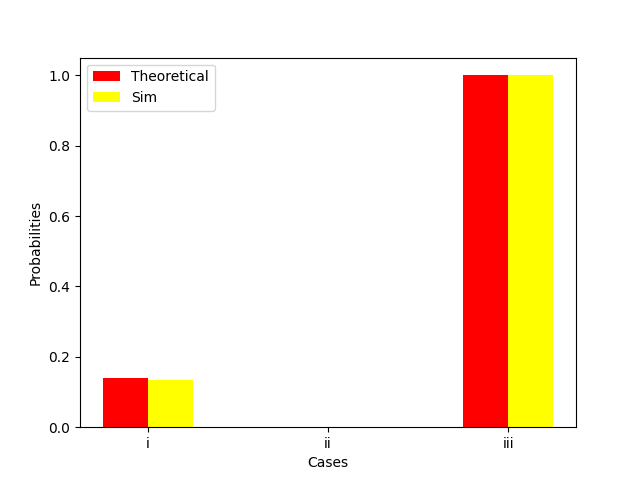
\includegraphics[width=\linewidth]{figure/plot}
 

\end{document}
